\documentclass[paper=a4, fontsize=11pt]{scrartcl}
\usepackage[T1]{fontenc}
\usepackage{fourier}

\usepackage[english]{babel}															% English language/hyphenation
\usepackage[protrusion=true,expansion=true]{microtype}	
\usepackage{amsmath,amsfonts,amsthm} % Math packages
\usepackage[pdftex]{graphicx}	
\usepackage{url}
\usepackage{hyperref}

\usepackage{algorithm}
%\usepackage{algorithmicx}
\usepackage[noend]{algpseudocode}


%%% Custom sectioning
\usepackage{sectsty}
\allsectionsfont{\centering \normalfont\scshape}
\usepackage{subfigure}
\usepackage{comment}

\usepackage{amsthm}
\newtheorem{thm}{Theorem}
\newtheorem{lem}{Lemma}

%%% Custom headers/footers (fancyhdr package)
\usepackage{fancyhdr}
\pagestyle{fancyplain}
\fancyhead{}											% No page header
\fancyfoot[L]{}											% Empty 
\fancyfoot[C]{}											% Empty
\fancyfoot[R]{\thepage}									% Pagenumbering
\renewcommand{\headrulewidth}{0pt}			% Remove header underlines
\renewcommand{\footrulewidth}{0pt}				% Remove footer underlines
\setlength{\headheight}{13.6pt}


%%% Equation and float numbering
%\numberwithin{equation}{section}		% Equationnumbering: section.eq#
%\numberwithin{figure}{section}			% Figurenumbering: section.fig#
%\numberwithin{table}{section}				% Tablenumbering: section.tab#


%%% Maketitle metadata
\newcommand{\horrule}[1]{\rule{\linewidth}{#1}} 	% Horizontal rule

\title{
		%\vspace{-1in} 	
		%\usefont{OT1}{bch}{b}{n}
		%\normalfont \normalsize \textsc{CS660 - Computer Networks} \\ [25pt]
		\normalfont
		\horrule{0.5pt} \\[0.4cm]
		\huge MORRF$^{*}$ : Sampling-Based Multi-Objective Motion Planning \\
		\horrule{2pt} \\[0.5cm]
}
\author{
		\normalfont %\normalsize
        Daqing Yi \\
}
%\date{}


%%% Begin document
\begin{document}
\maketitle

\section{Introduction}

\section{Related works}

\section{MORRF$^{*}$}

\subsection{Decomposition based multi-objective optimization}


\begin{thm}
\label{thm:moo-d:rrt}
The decomposition method is applicable to a RRT structure.
\begin{proof}
Let the path from start to goal with the most vertices be $ N $ segments.
Any other paths can be represented into $ N $ segments (because they have less than $ N $ segment).
By this way, all the paths could be mapped into a $ N $ dimensional space.
\end{proof}
\end{thm}

Given a multi-objective optimization problem with $ K $ objectives,
there are $ K $ objectives to be minimized. 
By Theorem \ref{thm:moo-d:rrt}, it can be decomposed into $ N $ subproblems.

Two types of tree structure are used for the optimization process.
\begin{itemize}
\item Each \emph{reference tree} explores for a single objective $ f_{k} (x), k \in K $. 
\item Each \emph{subproblem tree} explores for a subproblem $ g_{n} ( x \mid \lambda_{n} , z^{*} ) , n \in N $.
\end{itemize}

Like all the sampling-based optimization, the random positions are uniformly sampled from the workspace.
It means that all the tree have equivalent vertices constructed from same positions set sequentially.
But they are connected by different measurements of the costs, either a single objective or a cost from subproblem definition.
The edges of the trees can be different.

\begin{figure}
\centering
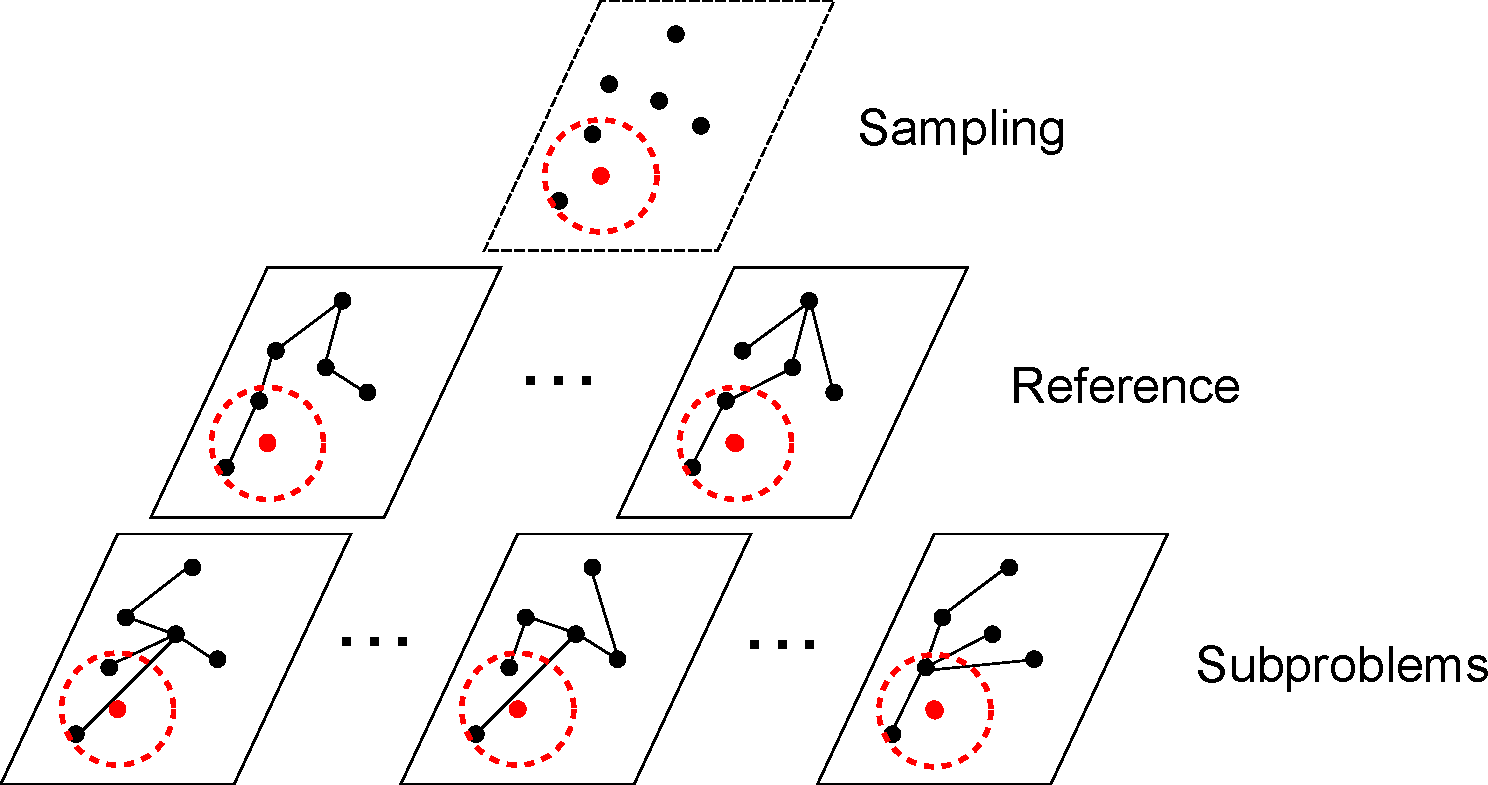
\includegraphics[width=0.7\linewidth]{./fig/MORRTstar}
\caption{Rapidly Exploring Process}
\label{fig:MORRTstar}
\end{figure}


\begin{algorithm}
\begin{algorithmic}[1]
\For{ \textbf{each} $ V_{r} \in \mathbf{V}_{r} $ } 
	\State $ V_{r} \leftarrow \{ x_{init} \} $; $ E_{r} \leftarrow \emptyset $; $ i \leftarrow 0 $
\EndFor
\For{ \textbf{each} $ V_{s} \in \mathbf{V}_{s} $ } 
	\State $ V_{s} \leftarrow \{ x_{init} \} $; $ E_{s} \leftarrow \emptyset $; $ i \leftarrow 0 $
\EndFor
\While{ $ i < N $ }
	\For{ \textbf{each} $ G_{r} \in \mathbf{G}_{r} $ } 
		\State $ G_{r} \leftarrow (V_{r}, E_{r}) $
	\EndFor
	\For{ \textbf{each} $ G_{s} \in \mathbf{G}_{s} $ } 
		\State $ G_{s} \leftarrow (V_{s}, E_{s}) $
	\EndFor
	\State $ x_{rand} \leftarrow $ \Call{ Sample }{$ i $} ; $ i \leftarrow i + 1 $
	\State $ V' \leftarrow V $; $ E' \leftarrow E $
	\State $ x_{nearest} \leftarrow $ \Call{Nearest}{$ G, x $}
	\State $ x_{new} \leftarrow $ \Call{Steer}{$ x_{nearest}, x $}
	\If{ \Call{ObstacleFree}{$ x_{nearest}, x_{new} $} }
		\For{ \textbf{each} $ G_{r} \in \mathbf{G}_{r} $ } 
		\State $ (V_{r}, E_{r}) \leftarrow $ \Call{ Extend$_{Ref}$ }{$ G_{r}, x_{new} $}
		\EndFor
		\For{ \textbf{each} $ G_{s} \in \mathbf{G}_{s} $ } 
		\State $ (V_{s}, E_{s}) \leftarrow $ \Call{ Extend$_{Sub}$ }{$ G_{s}, x_{new} $}
		\EndFor
	\EndIf
\EndWhile
\end{algorithmic}
\label{alg:rapidly_exploring_process}
\caption{Multi-objective Rapidly Random exploring }
\end{algorithm}

\begin{algorithm}
\begin{algorithmic}[1]
\State $ V' \leftarrow V' \cup \{ x_{new} \} $
\State $ x_{min} \leftarrow x_{nearest} $
\State $ X_{near} \leftarrow $ \Call{Near}{$ G, x_{new}, | V | $}
\For{\textbf{each} $ x_{near} \in X_{near} $ }
	\If{ \Call{ObstacleFree}{$ x_{new} , x_{near} $} }
		\State $ c_{k}' \leftarrow $ \Call{Cost$_{k}$}{$ x_{near} $} $ + c_{k}( $ \Call{Line}{$ x_{near}, x_{new} $} $ ) $ 
		\If{ $ c_{k}' < $ \Call{Cost$_{k}$}{$ x_{new} $} }
		\State $ x_{min} \leftarrow x_{near} $
		\EndIf
	\EndIf
\EndFor
\State $ E' \leftarrow E' \cup \{ ( x_{min}, x_{new} ) \} $
\For{\textbf{each} $ x_{near} \in X_{near} \setminus \{ x_{min} \} $ }
	\If{\Call{ObstacleFree}{$ x_{new} , x_{near} $}}
	    \State $ c_{k}' \leftarrow $ \Call{Cost$_{k}$}{$ x_{new} $} $ + c_{k}( $ \Call{Line}{$ x_{new}, x_{near} $} $ ) $ 
	    \If{ $ c_{k}' < $ \Call{Cost$_{k}$}{$ x_{near} $} }
			\State $ x_{parent} \leftarrow $ \Call{Parent}{$ x_{near} $}
			\State $ E' \leftarrow E' \setminus \{ ( x_{parent}, x_{near} ) \} $
			\State $ E' \leftarrow E' \cup \{ ( x_{new}, x_{near} ) \} $
		\EndIf
	\EndIf
\EndFor
\Return $ G' = (V', E') $ 
\end{algorithmic}
\label{alg:morrtstar:extend:ref}
\caption{ $ \mbox{Extend}_{Ref} (G, x) $}
\end{algorithm} 

\begin{algorithm}
\begin{algorithmic}[1]
\State $ V' \leftarrow V' \cup \{ x_{new} \} $
\State $ x_{min} \leftarrow x_{nearest} $
\State $ X_{near} \leftarrow $ \Call{Near}{$ G, x_{new}, | V | $}
\For{\textbf{each} $ x_{near} \in X_{near} $ }
	\If{ \Call{ObstacleFree}{$ x_{new} , x_{near} $} }
		\State $ \vec{c}' \leftarrow $ \Call{Cost}{$ x_{near} $} $ + \vec{c}( $ \Call{Line}{$ x_{near}, x_{new} $} $ ) $ 
		\State $ \eta' =  $ \Call{Fitness}{ $ \vec{c}' , \vec{c}^{*} \mid \lambda_{G} $ }
		\State $ \vec{c}_{new} = $ \Call{Cost}{$ x_{new} $} 
		\State $ \eta_{new} = $ \Call{Fitness}{ $ \vec{c}_{new} , \vec{c}^{*} \mid \lambda_{G} $ }
		\If{ $ \eta' < \eta_{new} $ }
			\State $ x_{min} \leftarrow x_{near} $
		\EndIf
	\EndIf
\EndFor
\State $ E' \leftarrow E' \cup \{ ( x_{min}, x_{new} ) \} $
\For{\textbf{each} $ x_{near} \in X_{near} \setminus \{ x_{min} \} $ }
	\If{\Call{ObstacleFree}{$ x_{new} , x_{near} $} }
		\State $ \vec{c}' \leftarrow $ \Call{Cost}{$ x_{new} $} $ + \vec{c}( $ \Call{Line}{$ x_{new}, x_{near} $} $ ) $ 
		\State $ \eta' =  $ \Call{Fitness}{ $ \vec{c}' , \vec{c}^{*} \mid \lambda_{G} $ }
		\State $ \vec{c}_{near} = $ \Call{Cost}{$ x_{near} $} 
		\State $ \eta_{near} = $ \Call{Fitness}{ $ \vec{c}_{near} , \vec{c}^{*} \mid \lambda_{G} $ }
		\If{ $ \eta' < \eta_{near} $ }
			\State $ x_{parent} \leftarrow $ \Call{Parent}{$ x_{near} $}
			\State $ E' \leftarrow E' \setminus \{ ( x_{parent}, x_{near} ) \} $
			\State $ E' \leftarrow E' \cup \{ ( x_{new}, x_{near} ) \} $
		\EndIf
	\EndIf
\EndFor
\Return $ G' = (V', E') $ 
\end{algorithmic}
\label{alg:morrtstar:extend:sub}
\caption{ $ \mbox{Extend}_{Sub} (G, x) $}
\end{algorithm} 

\section{Asymptotically optimality}

\begin{lem}
\label{lem:ref_tree:conv}
The reference tree will converge.
\begin{proof}
Haha
\end{proof}
\end{lem}

\begin{lem}
\label{lem:sub_tree:conv}
The subproblem tree will converge.
\begin{proof}
Baba
\end{proof}
\end{lem}

\begin{thm}
\label{thm:morrt:asym_opt}
\end{thm}


\bibliography{reference}
\bibliographystyle{plain}

\end{document}